%!TEX program = xelatex
%!TEX root = ../../theory.tex

\documentclass[a4paper, openany, oneside]{memoir}
\usepackage[no-math]{fontspec}
\usepackage{pgfplots}
\pgfplotsset{compat=newest}
\usepackage{commath}
\usepackage{mathtools}
\usepackage{amssymb}
\usepackage{amsthm}
\usepackage{booktabs}
\usepackage{mathtools}
\usepackage{xcolor}
\usepackage[separate-uncertainty=true, per-mode=symbol]{siunitx}
\usepackage[noabbrev, capitalize]{cleveref}
\usepackage{listings}
\usepackage[american inductor, european resistor]{circuitikz}
\usepackage{amsmath}
\usepackage{amsfonts}
\usepackage{ifxetex}
\usepackage[dutch,english]{babel}
\usepackage[backend=bibtexu,texencoding=utf8,bibencoding=utf8,style=ieee,sortlocale=en_GB,language=auto]{biblatex}
\usepackage[strict,autostyle]{csquotes}
\usepackage{parskip}
\usepackage{import}
\usepackage{standalone}
\usepackage{hyperref}
%\usepackage[toc,title,titletoc]{appendix}

\ifxetex{} % Fonts laden in het geval dat je met Xetex compiled
    \usepackage{fontspec}
    \defaultfontfeatures{Ligatures=TeX} % To support LaTeX quoting style
    \setromanfont{Palatino Linotype} % Tover ergens in Font mapje in root.
    \setmonofont{Source Code Pro}
\else % Terug val in standaard pdflatex tool chain. Geen ondersteuning voor OTT fonts
    \usepackage[T1]{fontenc}
    \usepackage[utf8]{inputenc}
\fi
\newcommand{\references}[1]{\begin{flushright}{#1}\end{flushright}}
\renewcommand{\vec}[1]{\boldsymbol{\mathbf{#1}}}
\newcommand{\uvec}[1]{\boldsymbol{\hat{\vec{#1}}}}
\newcommand{\mat}[1]{\boldsymbol{\mathbf{#1}}}
\newcommand{\fasor}[1]{\boldsymbol{\tilde{\vec{#1}}}}
\newcommand{\cmplx}[0]{\mathrm{j}}
\renewcommand{\Re}[0]{\operatorname{Re}}
\newcommand{\Cov}{\operatorname{Cov}}
\newcommand{\Var}{\operatorname{Var}}
\newcommand{\proj}{\operatorname{proj}}
\newcommand{\Perp}{\operatorname{perp}}
\newcommand{\col}{\operatorname{col}}
\newcommand{\rect}{\operatorname{rect}}
\newcommand{\sinc}{\operatorname{sinc}}
\newcommand{\IT}{\operatorname{IT}}
\newcommand{\F}{\mathcal{F}}

\newtheorem{definition}{Definition}
\newtheorem{theorem}{Theorem}


\DeclareSIUnit{\voltampere}{VA} %apparent power
\DeclareSIUnit{\pii}{\ensuremath{\pi}}

\hypersetup{%setup hyperlinks
    colorlinks,
    citecolor=black,
    filecolor=black,
    linkcolor=black,
    urlcolor=black
}

% Example boxes
\usepackage{fancybox}
\usepackage{framed}
\usepackage{adjustbox}
\newenvironment{simpages}%
{\AtBeginEnvironment{itemize}{\parskip=0pt\parsep=0pt\partopsep=0pt}
\def\FrameCommand{\fboxsep=.5\FrameSep\shadowbox}\MakeFramed{\FrameRestore}}%
{\endMakeFramed}

% Impulse train
\DeclareFontFamily{U}{wncy}{}
\DeclareFontShape{U}{wncy}{m}{n}{<->wncyr10}{}
\DeclareSymbolFont{mcy}{U}{wncy}{m}{n}
\DeclareMathSymbol{\Sha}{\mathord}{mcy}{"58}
\addbibresource{../../../../includes/bibliography.bib}

\begin{document}


\section{Main Analysis}

Let $L,N,M$ be integer parameters. Let $K\ge1$ be such that $KL$ is integer. Now $M$ cosets provide $KL$ out of $KLN$ samples of the input signal. Let $X[n]$ be a wide sense stationary stochastic process representing the input signal. Then let $\vec{x} \in \mathbb{C}^{KLN}$ be such that $(\vec{x})_i = X[i]$ for $i = 1,\ldots,KLN$. Let the deterministic correlation of $\vec{x}$ be given by $\vec{r}_x = \vec{x} \circ \vec{x}$.

During the main analysis, we will make use of two assumptions. Assume that
\begin{enumerate}
    \item[(1)] $X[i]=0$ for $ KLN-N+1 \le i \le KLN$ and
    \item[(2)] $R_X[i]=0$ for $|i| \ge LN-N$.
\end{enumerate}

The parameter $K$ will turn out to be related to the bias of the estimator of the autocorrelation of the input signal. Eventually, we will let $K \to \infty$, which will allow us to study the case in which an unbiased estimatior is used.

Let the sampling vector of coset $i$ be given by $\vec{c}_i \in \mathbb{C}^{N}$. The sampling vector relates the input signal to the output of a coset. Let the pseudo output of coset $i$ be given by $\vec{y}_i = \vec{c}_i \ast \vec{x}$. Let the output of coset $i$ be given by $\vec{y}'_i \in \mathbb{C}^{KL}$ such that $(\vec{y}'_i)_m=(\vec{y}_i)_{mN}$ for $m=1,\ldots,KL$. Then
\begin{align*}
    (\vec{y}'_i)_m &= (\vec{c}_i \ast \vec{x})_{mN} \\
    &= (\vec{x} \ast \vec{c}_i)_{mN} \\
    &= \sum_{k=1}^{KLN} (\vec{x})_k (\vec{c}_i)_{mN-k+1} \\
    &= \sum_{k=(m-1)N+1}^{mN} (\vec{x})_k (\vec{c}_i)_{mN-k+1} \\
    &= \sum_{k=1}^{N} (\vec{x})_{k+(m-1)N} (\vec{c}_i)_{N-k+1}.
\end{align*}
This shows the relationship between the sampling vector and the output of coset $i$. This relationship is depicted in \cref{fig:vis-yi}.

\begin{figure}
    \centering
    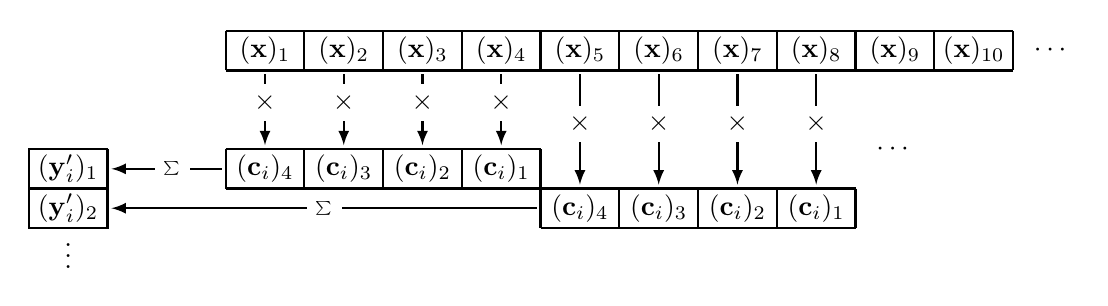
\begin{tikzpicture}
        \draw [black, thick] (-5,0.5) -- (5,0.5);
        \draw [black, thick] (-5,0) -- (5,0);

        \draw [black, thick] (-5,-1) -- (-1,-1);
        \draw [black, thick] (-5,-1.5) -- (-1,-1.5);
        \draw [black, thick] (-1,-1.5) -- (3,-1.5);
        \draw [black, thick] (-1,-2) -- (3,-2);
        \foreach \i in {-5,...,5} {
            \draw [black, thick] (\i, 0) -- (\i, 0.5);
        }
        \foreach \i in {1,...,10} {
            \draw ({\i-5.5},0.25) node[black] {$(\vec{x})_{\i}$};
        }

        \foreach \i in {-5,...,-1} {
            \draw [black, thick] (\i, -1) -- (\i, -1.5);
        }
        \foreach \i in {-5,...,-1} {
            \draw [black, thick] (\i+4, -1.5) -- (\i+4, -2);
        }
        
        \foreach \i in {4,...,1} {
            \draw ({(5-\i)-5.5},-1.25) node[black] {$(\vec{c}_i)_{\i}$};
        }
        \foreach \i in {4,...,1} {
            \draw ({(5-\i)-1.5},-1.75) node[black] {$(\vec{c}_i)_{\i}$};
        }
        \draw (3.5,-1) node[black] {$\cdots$};
        \draw (5.5,0.25) node[black] {$\cdots$};

        \foreach \i in {-5,...,-2} {
            \draw [black, thick, >=latex, ->] (\i+0.5,-0.05) -- node[pos=0.4,fill=white] {$\times$} (\i+0.5,-0.95);
        }
        \foreach \i in {-1,...,2} {
            \draw [black, thick, >=latex, ->] (\i+0.5,-0.05) -- node[pos=0.45,fill=white] {$\times$} (\i+0.5,-1.45);
        }
        \draw [black, thick, >=latex, ->] (-5.05,-1.25) -- node[pos=0.45,fill=white] {\tiny$\sum$} (-6.45,-1.25);
        \draw [black, thick, >=latex, ->] (-1.05,-1.75) -- node[pos=0.5,fill=white] {\tiny$\sum$} (-6.45,-1.75);
        \draw [black, thick] (-6.5,-1) -- (-6.5,-1.5) -- (-7.5,-1.5) -- (-7.5,-1) -- (-6.5,-1);
        \draw [black, thick] (-6.5,-1.5) -- (-6.5,-2) -- (-7.5,-2) -- (-7.5,-1.5) -- (-6.5,-1.5);
        \draw (-7,-1.25) node[black] {$(\vec{y}'_i)_1$};
        \draw (-7,-1.75) node[black] {$(\vec{y}'_i)_2$};
        \draw (-7,-2.25) node[black] {$\vdots$};
    \end{tikzpicture}
    \caption{Visualisation of $(\vec{y}_i)_1$ and $(\vec{y}_i)_2$ in the case that $N=4$}
    \label{fig:vis-yi}
\end{figure}

Consider the case that $\vec{c}_i = \begin{bmatrix}0 & 1 & 0 & 0\end{bmatrix}^T$. Then coset $i$ provides every third sample of all consecutive groups of four samples of the input signal. This is visualised in \cref{fig:vis-yi-case}.

\begin{figure}
    \centering
    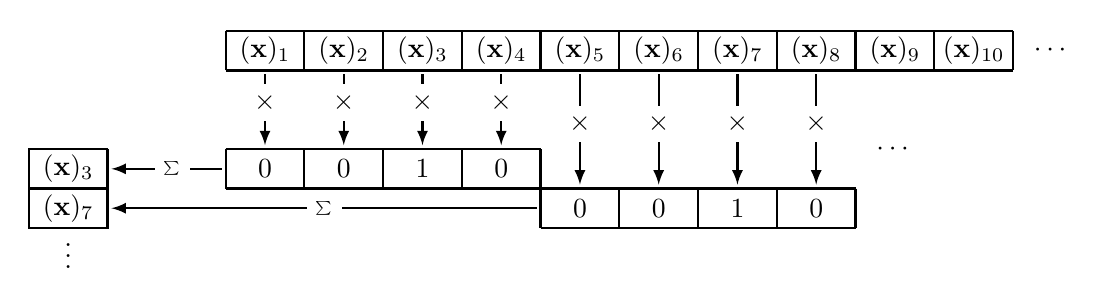
\begin{tikzpicture}
        \draw [black, thick] (-5,0.5) -- (5,0.5);
        \draw [black, thick] (-5,0) -- (5,0);

        \draw [black, thick] (-5,-1) -- (-1,-1);
        \draw [black, thick] (-5,-1.5) -- (-1,-1.5);
        \draw [black, thick] (-1,-1.5) -- (3,-1.5);
        \draw [black, thick] (-1,-2) -- (3,-2);
        \foreach \i in {-5,...,5} {
            \draw [black, thick] (\i, 0) -- (\i, 0.5);
        }
        \foreach \i in {1,...,10} {
            \draw ({\i-5.5},0.25) node[black] {$(\vec{x})_{\i}$};
        }

        \foreach \i in {-5,...,-1} {
            \draw [black, thick] (\i, -1) -- (\i, -1.5);
        }
        \foreach \i in {-5,...,-1} {
            \draw [black, thick] (\i+4, -1.5) -- (\i+4, -2);
        }
        
        \draw (-4.5,-1.25) node[black] {$0$};
        \draw (-3.5,-1.25) node[black] {$0$};
        \draw (-2.5,-1.25) node[black] {$1$};
        \draw (-1.5,-1.25) node[black] {$0$};
        \draw (-0.5,-1.75) node[black] {$0$};
        \draw (0.5,-1.75) node[black] {$0$};
        \draw (1.5,-1.75) node[black] {$1$};
        \draw (2.5,-1.75) node[black] {$0$};
        \draw (3.5,-1) node[black] {$\cdots$};
        \draw (5.5,0.25) node[black] {$\cdots$};

        \foreach \i in {-5,...,-2} {
            \draw [black, thick, >=latex, ->] (\i+0.5,-0.05) -- node[pos=0.4,fill=white] {$\times$} (\i+0.5,-0.95);
        }
        \foreach \i in {-1,...,2} {
            \draw [black, thick, >=latex, ->] (\i+0.5,-0.05) -- node[pos=0.45,fill=white] {$\times$} (\i+0.5,-1.45);
        }
        \draw [black, thick, >=latex, ->] (-5.05,-1.25) -- node[pos=0.45,fill=white] {\tiny$\sum$} (-6.45,-1.25);
        \draw [black, thick, >=latex, ->] (-1.05,-1.75) -- node[pos=0.5,fill=white] {\tiny$\sum$} (-6.45,-1.75);
        \draw [black, thick] (-6.5,-1) -- (-6.5,-1.5) -- (-7.5,-1.5) -- (-7.5,-1) -- (-6.5,-1);
        \draw [black, thick] (-6.5,-1.5) -- (-6.5,-2) -- (-7.5,-2) -- (-7.5,-1.5) -- (-6.5,-1.5);
        \draw (-7,-1.25) node[black] {$(\vec{x})_3$};
        \draw (-7,-1.75) node[black] {$(\vec{x})_7$};
        \draw (-7,-2.25) node[black] {$\vdots$};
    \end{tikzpicture}
    \caption{Visualisation of the case that $\vec{c}_i$ is chosen such that coset $i$ provides every third sample of all consecutive groups of four samples of the input signal}
    \label{fig:vis-yi-case}
\end{figure}

Let the correlation of the sampling vectors of cosets $i$ and $j$ be given by $\vec{r}_{c_i,c_j} = \vec{c}_i \circ \vec{c}_j$ and let the correlation of the pseudo outputs of cosets $i$ and $j$ be given by $\vec{r}_{y_i,y_j} = \vec{y}_i \circ \vec{y}_j$. Furthermore, let the correlation of the outputs of cosets $i$ and $j$ be given by $\vec{r}_{y'_i,y'_j} = \vec{y}'_i \circ \vec{y}'_j$. The goal of the reconstruction method is to reconstruct the autocorrelation of the input signal using the cross-correlations of all outputs of the cosets. We start by relating a subvector of $\vec{r}_{y'_i,y'_j}$ to a subvector of $\vec{r}_x$.

\begin{blockTheorem} \label{th:convolution-correlation}
    \makebox[\textwidth]{\centering $(\vec{c}_i \ast \vec{x}) \circ (\vec{c}_j \ast \vec{x}) = (\vec{c}_i \circ \vec{c}_j) \ast (\vec{x} \circ \vec{x})$.} \nolinebreak
\end{blockTheorem}

By \cref{th:convolution-correlation},
\begin{align*}
    \vec{r}_{y_i,y_j} =(\vec{c}_i \ast \vec{x}) \circ (\vec{c}_j \ast \vec{x}) = (\vec{c}_i \circ \vec{c}_j) \ast (\vec{x} \circ \vec{x}) = \vec{r}_{c_i,c_j} \ast \vec{r}_x.
\end{align*}
Denote a truncated version of $\vec{r}_{y_i,y_j}$ by
\begin{align*}
    \hat{\vec{r}}_{y_i,y_j} = \vec{r}_{y_i,y_j}[KLN-LN+2N-1,KLN+LN-1]
\end{align*}
and a truncated version of $\vec{r}_x$ by
\begin{align*}
    \hat{\vec{r}}_x = \vec{r}_x [KLN-LN+1,KLN+LN-1].
\end{align*}
The truncated versions of $\vec{r}_x$ and $\vec{r}_{y_i,y_j}$ are visualised in \cref{fig:vis-trun}.
\usetikzlibrary{decorations.pathreplacing}
\begin{figure}
    \centering
    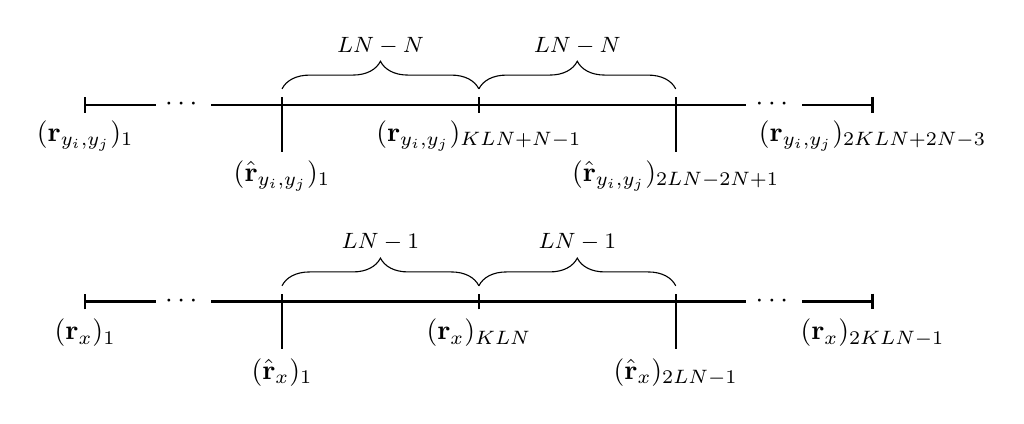
\begin{tikzpicture}
        \draw [black, thick] (-5,0) -- (5,0);
        \draw [black, thick] (-5,-0.1) -- (-5,0.1);
        \draw [black, thick] (5,0.1) -- (5,-0.1);
        \draw [black, thick] (-2.5,-0.6) -- (-2.5,0.1);
        \draw [black, thick] (0,-0.1) -- (0,0.1);
        \draw [black, thick] (2.5,-0.6) -- (2.5,0.1);
        \draw [decorate,decoration={brace,amplitude=10pt},yshift=0pt] (-2.5,0.2) -- (0,0.2) node [black,midway,yshift=0.55cm] {\footnotesize
        $LN-N$};
        \draw [decorate,decoration={brace,amplitude=10pt},yshift=0pt] (0,0.2) -- (2.5,0.2) node [black,midway,yshift=0.55cm] {\footnotesize
        $LN-N$};
        \draw (0,-0.4) node {$(\vec{r}_{y_i,y_j})_{KLN+N-1}$};
        \draw (-5,-0.4) node {$(\vec{r}_{y_i,y_j})_1$};
        \draw (5,-0.4) node {$(\vec{r}_{y_i,y_j})_{2KLN+2N-3}$};
        \draw (3.75,0) node[fill=white] {$\cdots$};
        \draw (-3.75,0) node[fill=white] {$\cdots$};
        \draw (-2.5,-0.9) node {$(\hat{\vec{r}}_{y_i,y_j})_1$};
        \draw (2.5,-0.9) node {$(\hat{\vec{r}}_{y_i,y_j})_{2LN-2N+1}$};

        \begin{scope}[shift={(0,-2.5)}]
            \draw [black, thick] (-5,0) -- (5,0);
            \draw [black, thick] (-5,-0.1) -- (-5,0.1);
            \draw [black, thick] (5,0.1) -- (5,-0.1);
            \draw [black, thick] (-2.5,-0.6) -- (-2.5,0.1);
            \draw [black, thick] (0,-0.1) -- (0,0.1);
            \draw [black, thick] (2.5,-0.6) -- (2.5,0.1);
            \draw [decorate,decoration={brace,amplitude=10pt},yshift=0pt] (-2.5,0.2) -- (0,0.2) node [black,midway,yshift=0.55cm] {\footnotesize
            $LN-1$};
            \draw [decorate,decoration={brace,amplitude=10pt},yshift=0pt] (0,0.2) -- (2.5,0.2) node [black,midway,yshift=0.55cm] {\footnotesize
            $LN-1$};
            \draw (0,-0.4) node {$(\vec{r}_{x})_{KLN}$};
            \draw (-5,-0.4) node {$(\vec{r}_{x})_1$};
            \draw (5,-0.4) node {$(\vec{r}_{x})_{2KLN-1}$};
            \draw (3.75,0) node[fill=white] {$\cdots$};
            \draw (-3.75,0) node[fill=white] {$\cdots$};
            \draw (-2.5,-0.9) node {$(\hat{\vec{r}}_{x})_1$};
            \draw (2.5,-0.9) node {$(\hat{\vec{r}}_{x})_{2LN-1}$};
        \end{scope}
    \end{tikzpicture}
    \caption{Visualisation of $\hat{\vec{r}}_x$ and $\hat{\vec{r}}_{y_i,y_j}$}
    \label{fig:vis-trun}
\end{figure}
Then
\begin{align*}
    \hat{\vec{r}}_{y_i,y_j}
    &= (\vec{r}_{c_i,c_j} \ast \vec{r}_x)[KLN-LN+2N-1,KLN+LN-1]\\
    &= (\vec{r}_x \ast \vec{r}_{c_i,c_j})[KLN-LN+2N-1,KLN+LN-1] \\
    &= \mat{R}_{c_i,c_j} \hat{\vec{r}}_x
\end{align*}
where $\mat{R}_{c_i,c_j}$ denotes the matrix
\begin{align*}
    \begin{bmatrix}
        (\vec{r}_{c_i,c_j})_{2N-1} & (\vec{r}_{c_i,c_j})_{2N-2} & \cdots & (\vec{r}_{c_i,c_j})_{1 }& 0 &  \cdots  \\
        0 & (\vec{r}_{c_i,c_j})_{2N-1} & \cdots & (\vec{r}_{c_i,c_j})_{2}& (\vec{r}_{c_i,c_j})_{1}  &\cdots  \\
        &&\multicolumn{2}{c}{\ddots} \\
        \cdots&(\vec{r}_{c_i,c_j})_{2N-1}&(\vec{r}_{c_i,c_j})_{2N-2}& \cdots & (\vec{r}_{c_i,c_j})_{1} & 0 \\
        \cdots&0&(\vec{r}_{c_i,c_j})_{2N-1}& \cdots & (\vec{r}_{c_i,c_j})_{2} & (\vec{r}_{c_i,c_j})_{1}
    \end{bmatrix}.
\end{align*}

Since we have related $\hat{\vec{r}}_{y_i,y_j}$ to $\hat{\vec{r}}_x$, we now make effort to relate a subvector of $\vec{r}_{y'_i,y'_j}$ to $\hat{\vec{r}}_{y_i,y_j}$. To this end, let the $2L-1\times 2LN-2N+1$ decimation matrix be defined by $(\mat{D})_{i,(i-1)N+1} = 1$ for $i=1,\ldots,2L-1$ and otherwise zero. Let the decimated truncated correlation of the pseudo outputs of cosets $i$ and $j$ be given by $\hat{\vec{r}}'_{y_i,y_j} = \mat{D} \hat{\vec{r}}_{y_i,y_j}$. Denote a truncated version of $\vec{r}_{y'_i,y'_j}$ by
\begin{align*}
    \hat{\vec{r}}_{y'_i,y'_j}=\vec{r}_{y'_i,y'_j}[KL-L+1,KL+L-1].
\end{align*}
The following theorem relates $\hat{\vec{r}}_{y'_i,y'_j}$ to $\hat{\vec{r}}'_{y_i,y_j}$.

\begin{blockTheorem} \lab{th:decimation-correlation}
    % Let $Y_i[n]$ and $Y_j[n]$ be wide sense stationary stochastic processes such that $(\vec{y}_i)_m = Y_i[m]$ and $(\vec{y}_j)_m = Y_j[m]$ for $m=1,\ldots,KLN$. Furthermore, let $Y'_i[n]$ and $Y'_j[n]$ be wide sense stationary stochastic processes such that $(\vec{y}'_i)_m = Y'_i[m]$ and $(\vec{y}'_j)_m = Y'_j[m]$ for $m=1,\ldots,KL$.
    % Assume that $\vec{x}$ is zero for the last $N-1$ elements.
    \makebox[\linewidth]{
        $\displaystyle E(N\hat{\vec{r}}_{y'_i,y'_j}) = E(\hat{\vec{r}}'_{y_i,y_j}).$
    } \nolinebreak
\end{blockTheorem}

Finally, we relate $\hat{\vec{r}}_x$ to the autocorrelation of the input signal and $\hat{\vec{r}}_{y'_i,y'_j}$ to the cross-correlation of the outputs of cosets $i$ and $j$. To do this, we identify the expected value of $\hat{\vec{r}}_x$ and $\hat{\vec{r}}_{y'_i,y'_j}$.

Let $\vecsc{r}_x \in \mathbb{C}^{2LN-1}$ be such that $(\vecsc{r}_x)_{i+LN} = R_X[i]$ for $i = -LN + N, LN-N$ and let $\vecsc{r}_{y'_i,y'_j} \in \mathbb{C}^{2L-1}$ be such that $(\vecsc{r}_{y'_i,y'_j})_{i+L}=R_{Y'_i,Y'_j}[i]$ for $i = -L+1,L-1$.
Note that $\vecsc{r}_x$ represents the autocorrelation of the input signal and that $\vecsc{r}_{y'_i,y'_j}$ represents the cross-correlation of the outputs of cosets $i$ and $j$.

By \cref{th:correlation-bias},
\begin{align*}
    E(\hat{\vec{r}}_x)[N,2LN-N] = \vec{b}_x \odot \vecsc{r}_x
\end{align*}
and
\begin{align*}
    E(\hat{\vec{r}}_{y'_i,y'_j}) =\vec{b}_{y'} \odot \vecsc{r}_{y'_i,y'_j}
\end{align*}
where
\begin{align*}
    \vec{b}_{x} =  \begin{bmatrix}
        (K-1)LN+1 \\
        (K-1)LN+2 \\
        \vdots \\
        KLN \\
        \vdots \\
        (K-1)LN+2 \\
        (K-1)LN+1
    \end{bmatrix} \text{ and }\vec{b}_{y'} = \begin{bmatrix}
        (K-1)L + 1 \\
        (K-1)L + 2 \\
        \vdots \\
        KL \\
        \vdots \\
        (K-1)L + 2 \\
        (K-1)L + 1
    \end{bmatrix}.
\end{align*}
Now $E(N\hat{\vec{r}}_{y'_i,y'_i}) = N\vec{b}_{y'} \odot \vecsc{r}_{y'_i,y'_i}$, whilst also
\begin{align*}
    E(N\hat{\vec{r}}_{y'_i,y'_i}) &= E(\hat{\vec{r}}'_{y_i,y_i}) \\
    &= \mat{D}\mat{R}_{c_i,c_j} E(\hat{\vec{r}}_x) \\
    &= (\mat{D}\mat{R}_{c_i,c_i})[N,2LN-N] E(\hat{\vec{r}}_x)[N,2LN-N] \\
    &= (\mat{D}\mat{R}_{c_i,c_i})[N,2LN-N] (\vec{b}_x \odot \vecsc{r}_{x})
\end{align*}
since, by \cref{th:correlation-bias}, $R_X[i]=0$ for $|i| \ge LN-N$ implies that $[E(\vec{r}_x)]_{m+KLN}=0$ for $|i| \ge LN-N$. Therefore equating and dividing by $KLN$ yields that
\begin{align*} 
    \left(\frac{\vec{b}_{y'}}{KL}\right) \odot \vecsc{r}_{y'_i,y'_j} =(\mat{D}\mat{R}_{c_i,c_i})[N,LN-N] \left[\left(\frac{\vec{b}_x}{KLN}\right) \odot \vecsc{r}_{x}\right].
\end{align*}
Equivalently,
\begin{align} \label{eq:bias-relationship}
    \vecsc{b}_{y'} \odot \vecsc{r}_{y'_i,y'_j} = (\mat{D} \mat{R}_{c_i,c_j})[N,LN-N] (\vecsc{b}_x \odot \vecsc{r}_x)
\end{align}
where $(\vecsc{b}_x)_i = (\vec{b}_x)_i/KLN$ for $i = 1,\ldots,2LN-1$ and $(\vecsc{b}_{y'})_i = (\vec{b}_{y'})_i/KL$ for $i = 1,\ldots,2L-1$. This equation relates the autocorrelation of the input signal to the cross-correlation of the outputs of cosets $i$ and $j$. However, this relationship involves element-wise multiplication, which shows that a biased estimate of $\vecsc{r}_{y'_i,y'_j}$ is related to a biased estimate of $\vecsc{r}_x$.

We now aggregate \cref{eq:bias-relationship} for all combinations of cosets. Let $\vecsc{b}_y$, $\vecsc{r}_y$ and $\vec{R}$ be such that
\begin{align}
    \vecsc{b}_y \odot \vecsc{r}_y \nonumber &= \begin{bmatrix}
        \vecsc{b}_{y'} \\ \vdots \\ \vecsc{b}_{y'}
    \end{bmatrix} \odot \begin{bmatrix}
        \vecsc{r}_{y'_1,y'_1} \\ \vdots \\ \vecsc{r}_{y'_M,y'_M}
    \end{bmatrix} \nonumber \\
    &= \begin{bmatrix}
        \vecsc{b}_{y'} \odot \vecsc{r}_{y'_1,y'_1} \\ \vdots \\ \vecsc{b}_{y'} \odot \vecsc{r}_{y'_M,y'_M}
    \end{bmatrix} \nonumber \\
    &= \begin{bmatrix}
        \mat{D}\mat{R}_{c_1,c_1} \\ \vdots \\ \mat{D}\mat{R}_{c_M,c_M}
    \end{bmatrix}[LN-N] (\vecsc{b}_x \odot \vecsc{r}_x) \nonumber \\
    &= \mat{R} (\vecsc{b}_x \odot \vecsc{r}_x). \label{eq:relationship-biased-aggregated}
\end{align}
It is important to notice that $\mat{R}$ in an $M^2(2L-1)\times 2LN-2N+1$ matrix. This means that \cref{eq:relationship-biased-aggregated} may be invertible, dependent on whether $\mat{R}$ has full column rank.


\subsection{Aymptotic}
It is important to notice that in \cref{eq:relationship-biased-aggregated} only $\vecsc{b}_x$ and $\vecsc{b}_y$ depend on $K$. This is remarkable, since this implies that $\mat{R}$ can be used to relate the estimates of $\vecsc{r}_x$ and $\vecsc{r}_{y}$ biased by $\vecsc{b}_x$ and $\vecsc{b}_y$ for any $K$. Furthermore, this means that the relationship still holds when $K \to \infty$. Let $K \to \infty$. Then $\vecsc{b}_x \to \vec{1}_{2LN-1}$ and $\vecsc{b}_y \to \vec{1}_{2L-1}$. Therefore, we see that
\begin{align*}
    \vecsc{b}_y \odot \vecsc{r}_{y} \to \vec{1}_{2L-1}\odot \vecsc{r}_{y} = \vecsc{r}_{y}
\end{align*}
and
\begin{align*}
    \mat{R} (\vecsc{b}_x \odot \vecsc{r}_x)\to \mat{R} (\vec{1}_{2LN-1} \odot \vecsc{r}_x) = \mat{R} \vecsc{r}_x.
\end{align*}
So
\begin{align} \label{eq:relationship-unbiased}
    \vecsc{r}_{y} = \mat{R} \vecsc{r}_{x}.
\end{align}
This concludes the main analysis.

\end{document}